\chapter{Introduction to the OPUS GUI}

This section of the documentation provides a tutorial approach to using the
new The Graphical Interface (GUI) that has been added to the OPUS system as
of version 4.2.  This represents a substantial initiative to make UrbanSim
and OPUS more user-friendly and accessible to modelers and model users ---
by reducing the need for programming expertise to use the system
effectively to build, estimate, and use model systems for a range of
applications.  We think the GUI offers a substantial advance in usability,
and look forward to user feedback, and contributions from collaborators, to
continue building on this foundation.

Before starting the tutorial, please install Opus and UrbanSim on your
machine if you haven't already.  Installation instructions are in
Appendix~\ref{appendix:installation}.

\section{Main Features}

The GUI is cross-platform compatible, and has been developed using the open
source Qt4 library and the PyQt Python interface to it.  Screenshots
included in this section will be taken from all three platforms, to give a
sense of the look and feel of the GUI on each platform.  After launching
the GUI from any of these platforms, the main Opus GUI window should be
displayed as in Figure \ref{fig:opus1-linux} or \ref{fig:opus1-mac}.

The organization of the GUI is based on an expectation that the work flow
for developing and using models can be effectively organized into tasks
that follow an ordering of data management, model management, scenario
management, and results management.  The main window of the GUI reflects
this work flow expectation, by implementing four tabs in the left-hand
panel of the main window labeled \emph{Data}, \emph{Models},
\emph{Scenarios}, and \emph{Results}, plus a \emph{General} tab.  Each of
the four tabs provides a container for configuring and running a variety of
tasks, organized into the main functional areas involved in developing and
using a simulation model.

\squishlist
\item The \emph{Data} tab organizes the processes related to moving data
  between the Opus environment and, doing data processing both within Opus,
  and also remotely in a database or GIS environment.  Opus can use Python
  to pass data and commands to a database system like Postgres or MS SQL
  Server, or to a GIS system like ArcGIS or PostGIS.  Tasks can be
  organized in the Data Manager as scripts, and run as a batch, or
  alternatively, they may be run interactively.
\item The \emph{Models} tab organizes the work of developing, configuring,
  and estimating the parameters of models, and of combining models into a
  model system.
\item The \emph{Scenarios} tab organizes the tasks related to configuring a
  scenario of input assumptions, and to interact with a run management
  system to actually run simulations on scenarios.  Tools to monitor and
  interact with a running simulation are provided here.
\item The \emph{Results} tab provides the tools to explore results once one
  or more scenarios have been simulated.  It integrates an Indicator
  Framework that makes it possible to generate a variety of indicators, for
  diagnostic and for evaluation purposes.  It also provides functionality
  to visualize indicators as charts, maps, and tables, and to export
  results to other formats for use outside of Opus.  \squishend

To launch the Opus GUI, you will need to run a python script called
\file{opus.py} in the \file{/opus/src/opus\_gui} directory.\footnote{Note
  the use of forward slashes in the path.  On the Macintosh OS X and Linux
  operating systems, and in Python, forward slashes are used to indicate
  separations in the path components.  On Windows, backward slashes are
  used instead.  Python can actually use forward slashes and translate them
  appropriately on Windows or other operating systems as needed, so we will
  use the convention of forward slashes throughout the text, for
  generality.}  If you have used the Windows installer to install Opus,
then a Windows \texttt{Start} menu item has been added under the Opus menu
item under programs, so launching Opus is a simple as selecting the
\texttt{OpusGUI Opus} menu item.  If you did not use the installer, for
example, on OS X, or Linux, then open a command window or shell, change
directory to the \file{opus\_gui} directory and type \texttt{python
  opus.py}.  In Windows, you can also double-click on the \file{opus.py}
file in the \file{/opus/src/opus\_gui} directory to launch the GUI.

However it is launched, it will start from a command shell, and this
window remains active while Opus is running.  Do not attempt to quit
this window until after exiting the Opus GUI, or Opus will close also.  

\begin{figure}[htp]
\begin{center}
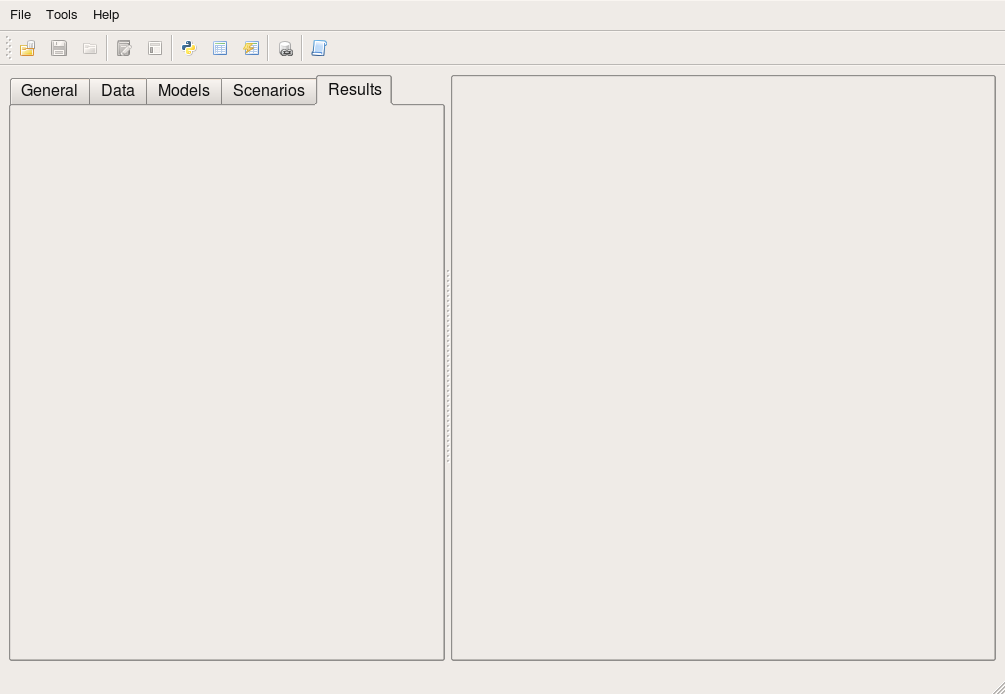
\includegraphics[scale=0.42]{part-gui/images/opus-startup.png}
\end{center}
\caption{Opus GUI Main Window - on Ubuntu Linux}
\label{fig:opus1-linux}
\end{figure}

\begin{figure}[htp]
\begin{center}
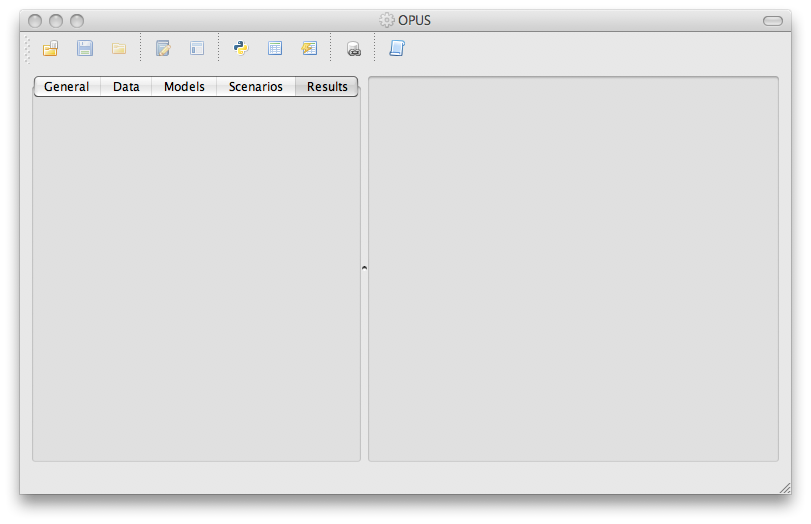
\includegraphics[scale=0.52]{part-gui/images/opus-startup-mac.png}
\end{center}
\caption{Opus GUI Main Window - on Leopard}
\label{fig:opus1-mac}
\end{figure}

\section{Introduction to XML-based Project Configurations}
\label{sec:intro-to-xml-based-project-configurations}

Notice that at this point there are no contents in any of the tabs.
Opus uses XML-based configuration files to flexibly specify the various
aspects of a project.  In addition, the appearance of the different tabs is
also driven from the XML configuration files, so that different parts of
the underlying functionality can be dynamically enabled and displayed, or
hidden.  XML stands for eXtensible Markup Language, and is a generalization
of the HTML markup language used to display web pages.  It is more
flexible, and has become widely used to store content in a structured form.

Let's add add content to the GUI by loading a \emph{Project}, which is in
fact, just an XML file containing configuration information.  From the main
menu, load a project from \file{eugene_gridcell.xml}, which is in the
default location of \file{opus/project_configs}.  The Opus window should
now appear as in Figure \ref{fig:opus2}.

\begin{figure}[htp]
\begin{center}
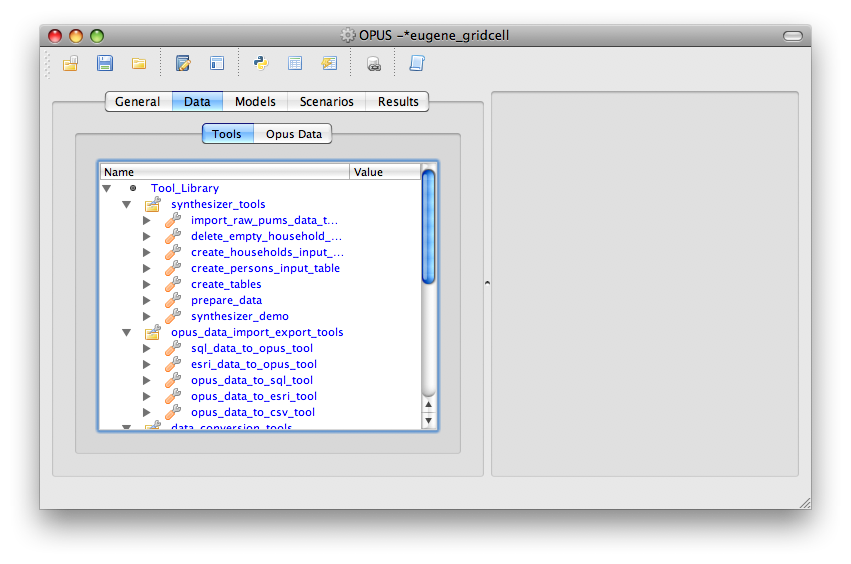
\includegraphics[scale=0.52]{part-gui/images/opus-open-project.png}
\end{center}
\caption{Opus GUI Main Window with eugene-gridcell Project Open}
\label{fig:opus2}
\end{figure}

One important property of XML project configurations is that they can
inherit from other project configurations.  In practical terms for a user,
this means that you can use default projects as templates, or parents, for
another project you want to create that is mostly the same as an existing
project, but has some changes from it.  The new project is called a
\emph{child} project.  By default, it inherits all the information
contained in the \emph{parent} project.  However, it can override any
information inherited from the parent, and add additional information.

Users should create their own projects in the \file{opus/project_configs}
directory.  This will allow them to keep projects localized in one place,
and to avoid editing and possibly corrupting one of the projects that are
in an Opus package in the source code tree.

In fact, the \file{eugene_gridcell.xml} configuration that we just opened
(in the default location of \file{opus/project_configs}) initially contains
almost no information of its own --- virtually everything is inherited from
a parent configuration.  As you edit and augment this configuration, more
information will be stored in the configuration.  It can be saved to disk
at any time using the ``Save'' or ``Save as \ldots'' commands on the
``File'' menu.

There is more information on XML-based project configurations later in this part
in Chapter \ref{chapter:xml-inheritance}, but the above information
should be enough to get started!
